\section{Introduction}

\subsection{Service overview}

A~fairly complete overview of the \LB service is given in \LB User's Guide~\cite{lbug}.
This section is a~brief excerpt only, providing minimal information necessary for
understanding the rest of this document.

The task of \LB is gathering \emph{\LB events} from various grid middleware components
(see Figure~\ref{f:comp-gather})
and delivering the events to \LB servers where users can query for them
(Figure~\ref{f:comp-query}).
%Figure~\ref{f:comp-gather} shows all principal components involved in the event gathering.

\begin{figure}[ht]
\centering
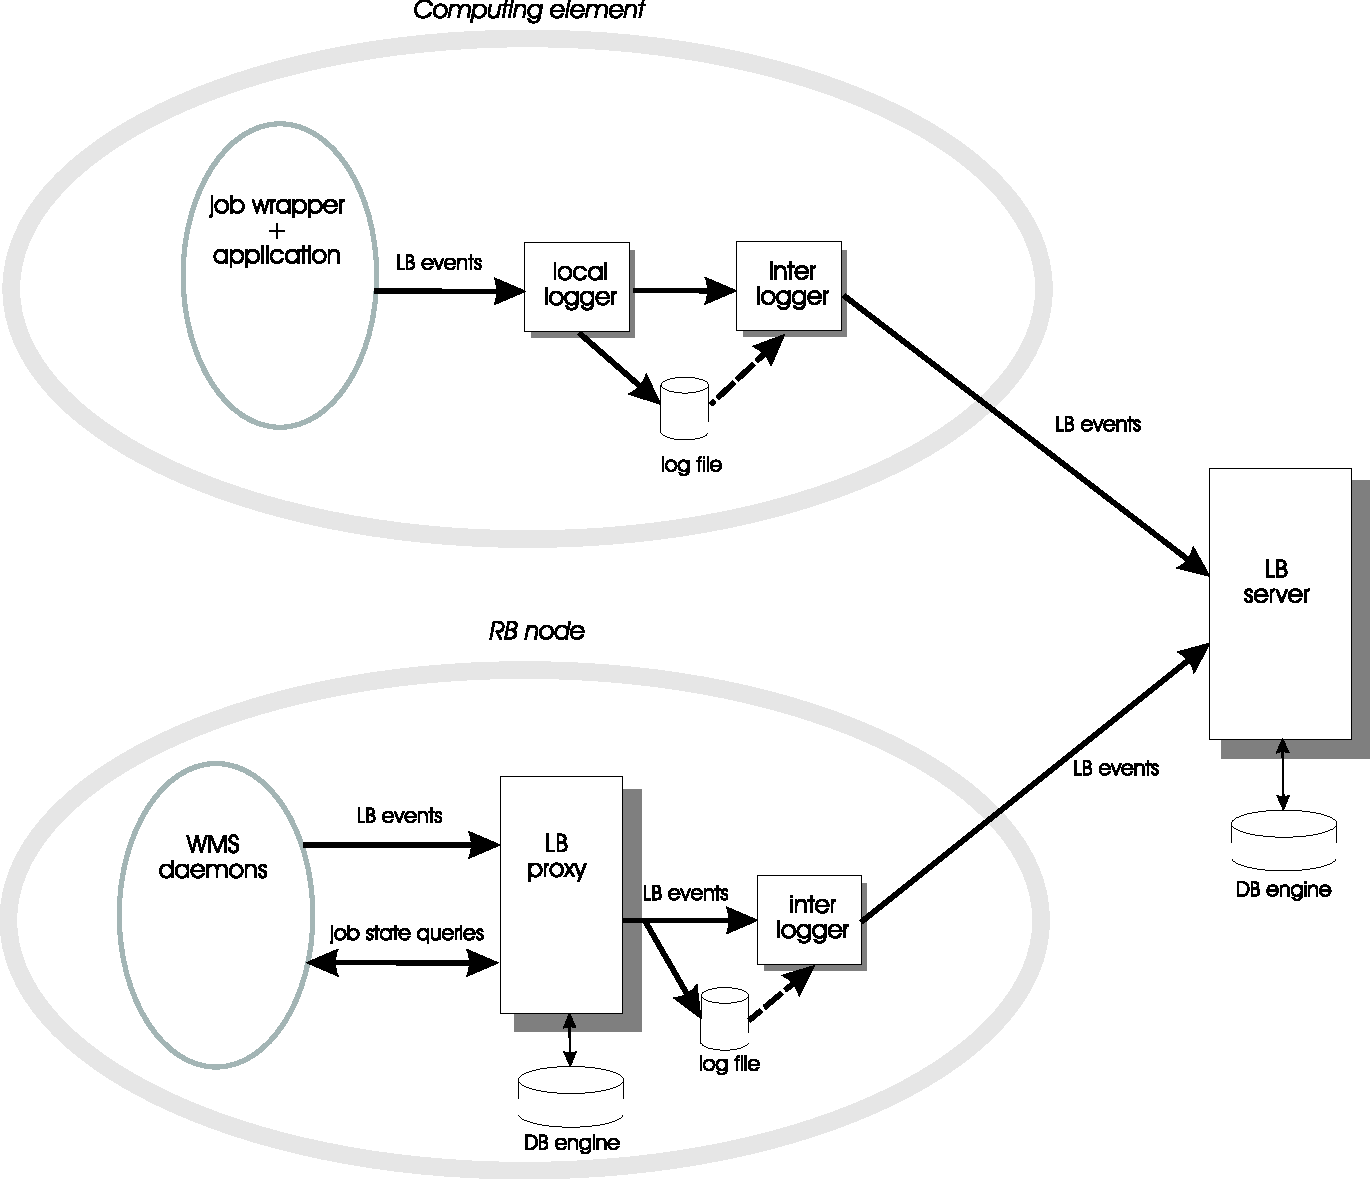
\includegraphics[width=.67\hsize]{LB-components-gather}
\caption{Components involved in gathering and transfering \LB events}
\label{f:comp-gather}
\end{figure}

\begin{figure}[ht]
\centering
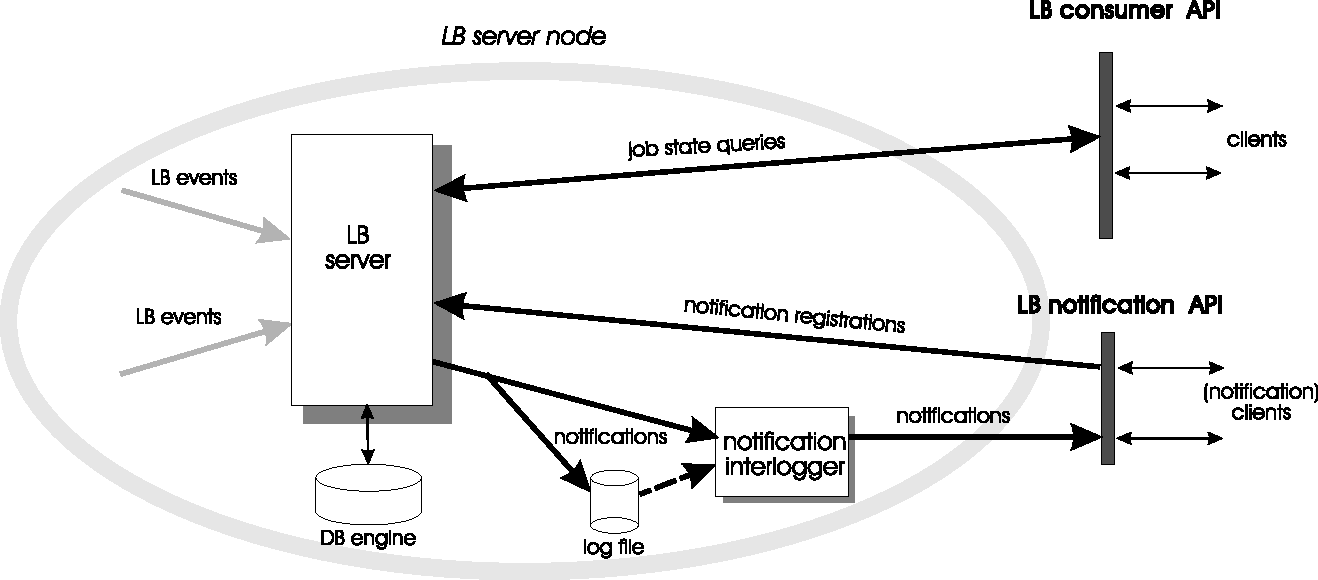
\includegraphics[width=.67\hsize]{LB-components-query}
\caption{\LB queries and notifications}
\label{f:comp-query}
\end{figure}

%\TODO{uplne to same (ty components) mame i v UG; chceme to tady duplikovat? 
%vlast kdyz v odstavci nad tim se pise, ze uz je to popsane v UG}
\input components


\subsection{Deployment scenarios}

%\TODO{salvet}

%\TODO{jakou zatez ktery snese}

\subsubsection{Standalone \LB server}
\label{deploy-stand}

This is the recommended standard production deployment.

\LB server is installed on a~dedicated machine,
where no other grid services (gLite WMS in particular) run.
Hence user queries and notification processing are offloaded 
from the WMS, not affecting its performance directly.

In this setup the full reported performance is achieved,
currently up to several hundreds thousands jobs per day, with the goal
of one million, see~\cite{lbtp}.

Further performance can be gained with clustering $M$ WMS's and $N$ \LB's
while configuring all WMS's to distribute jobs to the \LB's uniformly.
In this setup bottlenecks emerging from \LB proxy to \LB server serialized
communication are likely to be eliminated.
The optimal $M:N$ ratio strongly depends on the rate of user queries
and number of evaluated notifications,
and it must be determined empirically for each specific installation.

\subsubsection{Hybrid \LB server-proxy}
\label{deploy-hybrid}

\LB server runs on the WMS node, in combined server-proxy mode,
serving both user queries and supporting WMS.
Total processing requirements for a~single jobs are lower
(unlike with separated proxy and server, job state is computed and stored only once).

On the other hand, processing user queries is done on the WMS node,
limiting its performance then.
This setup is suitable for smaller installations with a~single (unclustered)
WMS, expected load of upto 30--50 kjobs/day, and not very heavy user-generated
load.

The functionality is available for \LBnew only.


\subsubsection{\LB server on WMS node}

\textbf{This setup is obsolete and very inefficient, hence discouraged.}

Ancient \LB versions, where \LB proxy was not available yet,
used to be frequently installed with \LB server on the WMS machine.
With the introduction of \LB proxy it makes little sense anymore
but, unfortunately, this setup still persists at some sites.
It's consequence is doubling both CPU and disk load, yielding observable
performance degradation.

Large production sites should consider standalone \LB server (Sect.~\ref{deploy-stand})
instead, while for smaller sites new hybrid setup (Sect.~\ref{deploy-hybrid}) may
be more appropriate.
